\documentclass[a4paper, 12pt]{article}

% \usepackage[utf8]{inputenc}
% \usepackage{tgtermes}
% \usepackage{fouriernc}
\usepackage[T1]{fontenc}
\usepackage[margin=3cm]{geometry}
\usepackage{babel}

\usepackage{biblatex}
\addbibresource{refs.bib}

\usepackage{amssymb}
\usepackage{amsmath}

\usepackage{ebproof}

\usepackage{enumerate}
\usepackage{verbatim}

\usepackage{xcolor}

\usepackage{listings}
\lstset{mathescape=true,
 xleftmargin=.25in}
\usepackage{quiver}

\usepackage[skip=10pt]{parskip}

\newcommand{\N}{\mathbb{N}}
\newcommand{\Z}{\mathbb{Z}}
\newcommand{\Q}{\mathbb{Q}}
\newcommand{\R}{\mathbb{R}}
\newcommand{\C}{\mathbb{C}}
\newcommand{\B}{\mathbb{B}}
\newcommand{\dif}{\mathrm{d}}
\newcommand{\Prop}{\mathit{Prop}}
\newcommand{\type}{\textsc{ Type}}
\newcommand{\Type}{\mathit{Type}}
\newcommand{\Sort}{\mathit{Sort\;}}
\renewcommand{\Prop}{\mathit{Prop}}
\DeclareMathOperator{\Arg}{Arg}
\DeclareMathOperator{\IN}{IN}
\DeclareMathOperator{\LT}{lt}
\DeclareMathOperator{\LM}{lm}
\DeclareMathOperator{\LC}{lc}
\DeclareMathOperator{\lcm}{lcm}
\newcommand{\la}[1]{\lambda{#1}.\,}


% Kan Danny godt lide
\usepackage[autostyle]{csquotes}
\usepackage{kpfonts}
% \usepackage{inconsolata}
\linespread{1.06}

\usepackage{minted}
\usemintedstyle{tango}
\setminted{fontsize=\footnotesize}
\setminted{breaklines}
\newcommand{\lean}[1]{\mintinline{lean}{#1}}

\usepackage{fontspec}
\setmonofont{JuliaMono}
\setmainfont{Linux Libertine O}
% \setmathfont[Digits, Latin]{Linux Biolinum O}

\usepackage{xcolor}
\usepackage{hyperref}
\hypersetup{%
	pdftitle=Mathematical project in Lean,
	pdfauthor={Andreas Bøgh Poulsen},
	colorlinks,
	linkcolor={red!50!black},
	citecolor={red!50!black},
	urlcolor={red!50!black},
	bookmarksnumbered=true
}

\usepackage[ntheorem]{mdframed}
\usepackage[amsmath,thmmarks,hyperref]{ntheorem}
\usepackage[capitalize]{cleveref}

% Frame for theorems
\definecolor{shadecolor}{gray}{0.93}
\definecolor{rulecolor}{gray}{0.4}
\mdfdefinestyle{thmframed}{%
	%usetwoside=false, % For use with memoir twoside
	skipabove=0.5em plus 0.4em minus 0.2em,
	skipbelow=0.5em plus 0.4em minus 0.2em,
	leftmargin=-7pt, rightmargin=-7pt, innerleftmargin=6pt,
	innerrightmargin=6pt, innertopmargin=6pt, innerbottommargin=3pt,
	% linewidth=1pt, linecolor=rulecolor, backgroundcolor=shadecolor,
  linewidth=1.5pt, linecolor=rulecolor, topline=false, bottomline=false, rightline=false, %leftmargin=1em,
	splittopskip=1.2em minus 0.2em,
	splitbottomskip=0.5em plus 0.2em minus 0.1em,
}
\mdfdefinestyle{thmempty}{
  usetwoside=false, % For use with memoir twoside
	skipabove=0.5em plus 0.4em minus 0.2em,
	skipbelow=0.5em plus 0.4em minus 0.2em,
	leftmargin=-7pt, rightmargin=-7pt, innerleftmargin=6pt,
	innerrightmargin=6pt, innertopmargin=6pt, innerbottommargin=3pt,
	% linewidth=1pt, linecolor=rulecolor, backgroundcolor=shadecolor,
  linewidth=1.5pt, linecolor=rulecolor, topline=false, bottomline=false, rightline=false,
	splittopskip=1.2em minus 0.2em,
	splitbottomskip=0.5em plus 0.2em minus 0.1em,
}

% New theorem style with a dot
\makeatletter
\newtheoremstyle{changedot}%
  {\item[\hskip\labelsep \theorem@headerfont ##2~~$\cdot$~~##1\theorem@separator]}%
  {\item[\hskip\labelsep \theorem@headerfont ##2~~$\cdot$~~##1\ (##3)\theorem@separator]}

\newtheoremstyle{changedotbreak}%
  {\item\hbox to \textwidth{\theorem@headerfont ##2~~$\cdot$~~##1\theorem@separator\hfill}}%
  {\item\hbox to \textwidth{\theorem@headerfont ##2~~$\cdot$~~##1\
      (##3)\theorem@separator\hfill}}
\makeatother

\theoremstyle{changedot}
\theoremseparator{.}
% \newmdtheoremenv[style=thmframed]{theorem}{Theorem}[section]
% \newmdtheoremenv[style=thmframed]{proposition}[theorem]{Proposition}
% \newmdtheoremenv[style=thmframed]{lemma}[theorem]{Lemma}
% \newmdtheoremenv[style=thmframed]{corollary}[theorem]{Corollary}
\newmdtheoremenv[style=thmempty]{theorem}{Theorem}[section]
\newmdtheoremenv[style=thmempty]{proposition}[theorem]{Proposition}
\newmdtheoremenv[style=thmempty]{lemma}[theorem]{Lemma}
\newmdtheoremenv[style=thmempty]{corollary}[theorem]{Corollary}
\newmdtheoremenv[style=thmempty]{example}[theorem]{Example}

\theorembodyfont{\normalfont}
%\theoremsymbol{\ensuremath{\triangle}}
\newmdtheoremenv[style=thmframed]{definition}[theorem]{Definition}

\theoremstyle{changedotbreak}
\newmdtheoremenv[style=thmframed]{definitionbreak}[theorem]{Definition}

\theoremstyle{nonumberplain}
\theoremheaderfont{\normalfont\itshape}
\theorembodyfont{\normalfont}
\theoremsymbol{\ensuremath{\square}}
\newtheorem{proof}{Proof}

\Crefname{theorem}{Theorem}{Theorems}
\Crefname{proposition}{Proposition}{Propositions}
\Crefname{lemma}{Lemma}{Lemmata}
\Crefname{corollary}{Corollary}{Corollaries}
\Crefname{definition}{Definition}{Definitions}

\crefformat{equation}{(#2#1#3)}

% / Kan Danny godt lide

% \usepackage[eng,exjobb]{KTHEEtitlepage}

\title{Parametric Gröbner bases\\{\large \textsc{Geometry \& applications}}}
\author{Andreas Bøgh Poulsen, student id: 201805425}

\newcommand*{\titleGM}{%\begingroup % Create the command for including the title page in the document
%\hbox{ % Horizontal box
\hspace*{0.2\textwidth} % Whitespace to the left of the title page
\rule{1pt}{\textheight} % Vertical line
\hspace*{0.05\textwidth} % Whitespace between the vertical line and title page text
\parbox[b]{0.75\textwidth}{ % Paragraph box which restricts text to less than the width of the page
{\noindent\Huge\bfseries  Parametric Gröbner bases\\{\large \textsc{Geometry \& applications}}\\}\\[2\baselineskip] % Title
{\large \textit{Andreas Bøgh Poulsen \hfill 201805425 }}\\%[1\baselineskip]
% {\large  } \\[4\baselineskip] % Tagline or further description
{\large } % Author name
\parbox[b][0pt]{0.5\textwidth}{
  \hspace{2cm}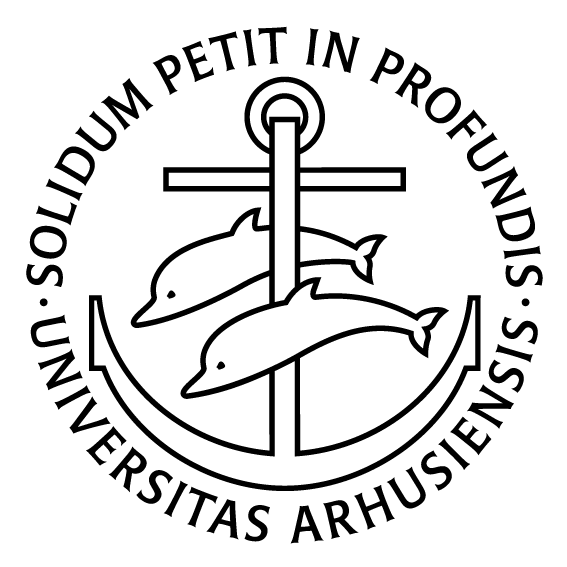
\includegraphics[width=0.5\textwidth]{ausegl_sort.png}
  \vspace{-10cm}
}

% \begin{centering}
  % 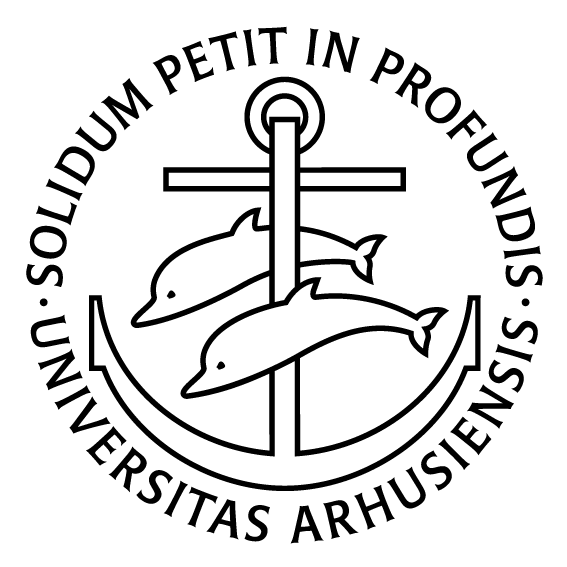
\includegraphics[width=0.5\textwidth]{ausegl_sort.png}
% \end{centering}
\vspace{0.5\textheight} % Whitespace between the title block and the publisher
\vfill
{\noindent Supervisor: Niels Lauritzen \hspace{2.5cm} 
\includegraphics{AU_logo.png}  }\\[\baselineskip] % Publisher and logo
}%}
% \endgroup
}

\begin{document}
% \maketitle
\titleGM
% \vfill
% Vejleder: Niels Lauritzen
% \strut\hfill
% 
\includegraphics[right]{AU_logo.png}
\newpage
\tableofcontents

\newpage

\section*{Introduction}


\section{Preliminaries}
This project will assume familiarity with ring theory, multivariate polynomials over fields. A familiarity with Gröbner bases will be beneficial, but we will introduce the necesary notations and definitions. Let $R$ be a Noetherian, commutative ring and $X = (x_{1}, x_{2}, \dots, x_{n})$ be an ordered collection of symbols. We denote the ring of polynomials in these variables $R[X]$. Given two (disjoint) sets of variables $X$ and $Y$, we will use $R[X, Y]$ to mean $R[X \cup Y]$, which is naturally isomorphic to $R[X][Y]$. A monomial is a product of variables and a term is a monomial times a coefficient. We denote a monomial as $X^{v}$ for some $v \in \N^{n}$.

\begin{definition}[Monomial order, leading term]
  A \textit{monomial order} is a total order $<$ on the set of monomials satisfying that $u < v \implies wu < wv$.

  Given a monomial order $<$ and a polynomial $f \in R[X]$, the \textit{leading term} of $f$ is the term with the largest monomial w.r.t. $<$ and is denoted by $\LT_{<}(f)$. If $\LT_{<}(f) = a\cdot m$ for some monomial $m$ and $a \in R$, then we denote $\LM_{<}(f) = m$ and $\LC_{<}(f) = a$. If $<$ is clear from context, it will be omitted.
\end{definition}

These definitions naturally extend to sets of polynomials, so given a set of polynomials $F \subset k[X]$, we denote $\LM_{<}(F) := \{\LM_{<}(f) \mid f \in F\}$. The above definitions work over a general ring (and we will use that), for from here, we'll work over a field $k$. With this, we can give the definition of a Gröbner basis.

\begin{definition}[Gröbner basis]
  Let $G \subset k[X]$ be a finite set of polynomials and $<$ be a monomial order. We say $G$ is a \textit{Gröbner basis} if
  $\langle \LT_{<}(G) \rangle = \LT_{<}(\langle G \rangle )$
\end{definition}

\section{Definitions and initial results}
The purpose of this project is to study parametric Gröbner bases, so let's introduce those. The bare concept is rather simple.

\begin{definition}[Parametric Gröbner basis]
  Let $k$, $k_{1}$ be fields, $U$ and $X$ be collections of variables and $F \subset k[U, X]$ be a finite set of polynomials. A \textit{parametric Gröbner basis} is a finite set of polynomials $G \subset k[U, X]$ such that $\sigma(G)$ is a Gröbner basis of $\langle \sigma(F) \rangle$ for any ring homomorphism $\sigma : k[U] \to k_{1}$.
\end{definition}

We call such a $\sigma : k[U] \to k_{1}$ a \textit{specialization}. By the linearity of $\sigma$, all such ring homomorphisms can be characterized by their image of $U$. Thus, we can identify $\{\sigma : k[U] \to k_{1} \mid \sigma \text{ is a ring hom.}\}$ with the affine space $k_{1}^{m}$ when $U$ has $m$ elements. For $\alpha \in k_{1}^{m}$ we'll denote the corresponding map
\[\sigma_{\alpha}(u_{i}) = \alpha_{i} \quad \text{for $u_{i} \in U$}\] extended linearly.

When we work with these parametric Gröbner bases, it will be more convenient to have a bit more information attached to them, namely which elements are required for which $\sigma$. Since $\sigma$ is described by an $\alpha \in k_{1}^{m}$, we can restrict them using subsets of $k_{1}^{m}$.

\begin{definition}[Vanishing sets \& algebraic sets]
  Let $E$ be a finite subset of $k[X]$. Then the \textit{vanishing set} of $E$ is $V(E) := \{v \in k^{n} \mid e(v) = 0 \;\; \forall e \in E\}$.

  An \textit{algebraic set} is a set of the form $V(E) \setminus V(N)$ for two finite subsets $E$ and $N$ of $k[X]$.
\end{definition}

\begin{definition}[Gröbner system]
  Let $A$ be an algebraic set and $G \subset k[U, X]$ be a finite set. Then $(A, G)$ is called a \textit{segment of a Gröbner system} if $\sigma_{\alpha}(G)$ is a Gröbner basis of $\sigma_{\alpha}(\langle G \rangle)$ for all $\alpha \in A$. A set $\{(A_{1}, G_{1}), \dots, (A_{t}, G_{t})\}$ is called a \textit{Gröbner system} if each $(A_{i}, G_{i})$ is a segment of a Gröbner system.
\end{definition}

\begin{example}
  Let $X = \{x, y\}$ and $U = \{u\}$ and consider the polynomials $f(x, y, u) = ux^{2} + x$ and $g(x, y, u) = xy + 1$. When $u \neq 0$, a Gröbner basis of $\langle f, g \rangle$ could be $(y-u, ux + 1)$, whatever $u$ may be. \colorbox{red}{TODO}
\end{example}

\colorbox{red}{Skriv om Kalkbrener}
\begin{definition}[Leading coefficient w.r.t. variables]
  Let $f \in k[U][X]$. Then the leading term of $f$ is denoted $\LT_{U}(f)$, the leading coefficient is $\LC_{U}(f)$ and the leading monomial is $\LM_{U}(f)$. These notations are also used when $f \in k[U, X]$, just viewing $f$ as a polynomial in $k[U][X]$.
\end{definition}

Note that $\LC_{U}(f) \in k[U]$, i.e. the leading term is a polynomial in $k[U]$ times a monomial in $X$.

From this point, we assume that the monomial order on $k[U, X]$ satisfies $x > u$ for all $x \in X$ and $u \in U$. This monomial order restricts to a monomial order on $k[X]$, denoted by $<_{X}$. Note that this assumption is not too restrictive, as both the lexicographic, reverse lexicographic and graded versions of those satisfies this assumption.

\begin{lemma}\label{lem:grb_iff_reduc_to_z}
  Let $G$ be a Gröbner basis of an ideal $\langle F \rangle$ w.r.t. $<$, let $\alpha \in k_{1}^{m}$ and set $G_{\alpha} := \{\sigma_{\alpha}(g) \in G \mid \sigma_{\alpha}(\LC_{U}(g)) \neq 0\} = \{g_{1}, g_{2}, \dots, g_{l}\} \subset k_{1}[X]$. Then $G_{\alpha}$ is a Gröbner basis of the ideal $\langle \sigma_{\alpha}(F) \rangle$ w.r.t. $<_{X}$ if and only if $\sigma_{\alpha}(g)$ is reducible to 0 modulo $G_{\alpha}$ for every $g \in G$.
\end{lemma}
\begin{proof}
  To we written after \colorbox{red}{Kalkbrener}
\end{proof}


We will use this lemma in a slightly different formulation:

% \begin{lemma}
%   Let $G = \{g_{1}, g_{2}, \dots, g_{k}\}$ be a Gröbner basis of an ideal $\langle F \rangle$ in $k[U, X]$ w.r.t $<$ and let $\alpha \in V(G \cap k[U])$. If $\sigma_{\alpha}(\LC_{U}(g)) \neq 0$ for each $g \in G \setminus (G \cap k[U])$, then $\sigma_{\alpha}(G)$ is a Gröbner basis of $\langle \sigma_{\alpha}(F) \rangle$.
% \end{lemma}
% \begin{proof}
%   Since $\alpha \in V(G \cap k[U])$ and $\LC_{U}(g) = g$ for any $g \in G \cap k[U]$, we have that $\sigma_{\alpha}(\LC_{U}(g)) = 0$ for all $g \in G \cap K[U]$. By assumption, $\sigma_{\alpha}(\LC_{U}(g)) \neq 0$ for any $g \notin G \cap k[U]$, thus $\sigma_{\alpha}(\LC_{U}(g)) = 0 \iff g \in G \cap k[U] \iff \sigma_{\alpha}(g) = 0$.

%   Now, $G_{\alpha} = \{\sigma_{\alpha}(g) \mid \sigma_{\alpha}(\LC_{U}(g)) \neq 0\}$ and take any $g \in G$. If $\sigma_{\alpha}(g) \in G_{\alpha}$, then $\LT(\sigma_{\alpha}(g)) = \sigma_{\alpha}(\LC_{U}(g)) \cdot \LM_{U}(g)$ since $x > u$ for all $x \in X$ and $u \in U$. Thus, $\sigma_{\alpha}(g)$ is reducible to $0$ modulo $G_{\alpha}$, since it's leading term is divisible by its own leading term.  On the other hand, if $\sigma_{\alpha}(g) \notin G_{\alpha}$, then $\sigma_{\alpha}(g) = 0$, so is immediately reducible to zero.
% \end{proof}


\begin{lemma}
  Let $G = \{g_{1}, g_{2}, \dots, g_{k}\}$ be a Gröbner basis of an ideal $\langle F \rangle$ in $k[U, X]$ w.r.t $<$ and let $\alpha \in k_{1}^{m}$. If $\sigma_{\alpha}(\LC_{U}(g)) \neq 0$ for each $g \in G \setminus (G \cap k[U])$, then $\sigma_{\alpha}(G)$ is a Gröbner basis of $\langle \sigma_{\alpha}(F) \rangle$.
\end{lemma}
\begin{proof}
  Let $G_{\alpha} = \{\sigma_{\alpha}(g) \mid \sigma_{\alpha}(\LC_{U}(g)) \neq 0\}$. If there is any $g \in G$, such that $\sigma_{\alpha}(g) \in k_{1} \setminus \{0\}$, then $g \in G \cap k[U]$ since $\sigma_{\alpha}(\LC_{U}(g)) \neq 0$ for all $g \in G \setminus K[U]$. Furthermore, since $g \in \langle F \rangle$, we get that $\langle \sigma_{\alpha}(F) \rangle = k_{1}[X]$ and $\sigma_{\alpha}(G)$ is a Gröbner basis.

  If there is no such $g$, then $\alpha \in V(G \cap k[U])$. Take any $g \in G$. If $\sigma_{\alpha}(g) \in G_{\alpha}$, then $\LT(\sigma_{\alpha}(g)) = \sigma_{\alpha}(\LC_{U}(g)) \cdot \LM_{U}(g)$ since $x > u$ for all $x \in X$ and $u \in U$. Thus, $\sigma_{\alpha}(g)$ is reducible to $0$ modulo $G_{\alpha}$, since it's leading term is divisible by its own leading term.  On the other hand, if $\sigma_{\alpha}(g) \notin G_{\alpha}$, then $\sigma_{\alpha}(g) = 0$, so is immediately reducible to zero. Thus $\sigma_{\alpha}(G)$ is a Gröbner basis of $\langle \sigma_{\alpha}(F) \rangle$ by lemma~\ref{lem:grb_iff_reduc_to_z}.
\end{proof}

With lemma~\ref{lem:grb_iff_reduc_to_z} in mind, we can start constructing Gröbner systems. Let $G$ be a reduced Gröbner basis of an ideal $\langle F \rangle \subset k[U, X]$, and let $H = \{\LC_{U}(g) \mid g \in G \setminus k[U]\}$. Then $\left(k_{1}^{m} \setminus \bigcup_{h \in H} V(h), G\right)$ is a segment of a Gröbner system. Thus, to make a Gröbner system, we need to find segments covering $\bigcup_{h \in H} V(h) = V(\lcm\{h \mid h \in H\})$.

If we take $G$ to be a reduced Gröbner basis, then $h \notin \langle F \rangle$ for any $h \in H$ since then the corresponding leading term would be divisible by a leading term in $G$. This is not allowed when $G$ is reduced. Hence, we can find a Gröbner basis $G_{1}$ of $F \cup \{h\}$, which will then form a segment $(k_{1}^{m} \setminus \bigcup_{h \in H_{1}} V(h), G_{1})$ where $H_{1} = \{\LC_{U}(g) \mid g \in G_{1}\}$. Since $k[U, X]$ is Noetherian, this will eventually stop, forming a Gröbner system.

This leads us to the first algorithm.


\section{Martin-Löf dependent type theory}\label{sec:tt}
Dependent type theory is a logical theory, comparable to first-order logic. Similarly to how we usually think we do mathematics in first-order logic with ZFC set theory on top, we can translate our mathematical theories into other logical theories. In this section, I'll explain how dependent type theory works as a formal system. The development will largely follow the exposition of \cite{rijke2022introduction}.

We'll build a dependent type theory, which is similar to the one used by Lean. The goal is not to match the calculus of inductive constructions (which is used in Lean), but rather to develop a theory together, to see how and why the choices Lean has made, make sense. If you're only interested in learning Lean, feel free to skip this section.

\subsection{Intuition and how to read the notation}
The following development may seem very notation-heavy and needlessly abstract, so here's a little primer: Suppose I have three functions (or morphisms)
\begin{align*}
  f &: A \to B \\
  g &: A \to C \\
  h &: B \to C
\end{align*}

The the composition $h \circ f : A \to C$ make sense, but the composition $h \circ g$ doesn't. Keeping track of domains and codomains in this small example is not a problem, but when more functions get involved, it can become unwieldy. This is where a type-checking compiler, as found in programming languages like Java and Haskell, can help.

Similarly, if we have three propositions
\begin{align*}
  p_{1} &= P \implies Q \\
  p_{2} &= P \implies R \\
  p_{3} &= Q \implies R
\end{align*}

have can deduce $P \implies R$ from $p_{1}$ and $p_{3}$, but we cannot deduce that from $p_{1}$ and $p_{2}$. This is similar to the situation above. In fact, we translate our propositions directly into functions and get a compiler to check it for us.

Now, most propositions are not fixed statements, they are parameterized by variables, for example $p_{4} = x \le 0$. Since the truth of this proposition is dependent on the element $x$, we can't translate it into any fixed type. So we extend the type theory of our programming language, so that types can depend on variables, then build a type-checker for this type theory, and then we get a checker for our propositions.

\subsubsection{Deduction rules}

The rules for our language are given by deduction rules. There are two types of deduction rules: typing rules and evaluation rules. The typing rules are only needed by the type checker. They are statements of the form \textit{``if $f : A \to B$ and $g : B \to C$ are functions with given domains and codomains, then $g \circ f : A \to C$ is a function with the given domain and codomain.''} Strictly speaking, this is all we need to formulate mathematics, as we only need the type checker. However, it will turn out to be useful to have an actual programming language. This means we need to define what $g \circ f$ does. This is given by an evaluation rule: \textit{``if $a \in A$ is an element and $f : A \to B$ and $g : B \to C$ are functions with given domains and codomains, then $(g \circ f)(a) = g(f(a))$.''} This tells us how to evaluate the terms we build. In the text below, rules that end in $A \type$ or $a : A$ are typing rules, and rules like $f(x) \doteq y$ are evaluation rules.

\subsection{Inference rules}
An inference rule is on the form

\begin{prooftree}
  \hypo{\Gamma \vdash P}
  \hypo{\Gamma \vdash Q}
  \infer2[$\land$-intro]{\Gamma \vdash P \land Q}
\end{prooftree}

which is read as follows: if we, in a context $\Gamma$, can prove $P$ and in the same context can prove $Q$, then we can prove $P \land Q$ in the context $\Gamma$.

The defining feature of {\emph type} theory is, that every element has a type. Thus the above is meaningless, as $P$ and $Q$ have no type. Compare this to ZFC, where everything is either a proposition from first-order logic, or a set. This leads to weird statements like $0 \in 1$, which is well-posed since everything is a set but does not carry meaning in our ``usual'' way of doing mathematics. Type theory asks that every element has a type. This is particularly helpful when doing computerized proofs, as it helps the proof-checker catch weird statements like $0 \in 1$. Since $1$ has the type of a natural number and not the type of a set, Lean can give an error, instead of silently trying to prove what may well have been a typo.

In type theory, the above rewrite rule would look like this:

\begin{prooftree}
  % \hypo{\Gamma \vdash \mathit{Prop} \type}
  \hypo{\Gamma \vdash P : \mathit{Prop}}
  \hypo{\Gamma \vdash Q : \mathit{Prop}}
  \infer2[$\land$-intro]{\Gamma \vdash P \land Q : \Prop}
\end{prooftree}

Everything is read the same, except $P : \Prop$ is read ``$P$ has type $\Prop$''. $\Prop$ is the type of propositions. I will not spend too much time going through every single inference rule. I will, however, introduce the defining features of dependent type theory: dependent types, and show how they are used.

\begin{definition}
  Type theory has four different \textit{judgments}.
  \begin{enumerate}
    \item $\Gamma \vdash A \type$ says $A$ is a well-formed type in context $\Gamma$.
    \item $\Gamma \vdash A \doteq B \type$ says $A$ and $B$ are judgementally equal types in context $\Gamma$.
    \item $\Gamma \vdash a : A$ says $a$ is an element of type $A$ in context $\Gamma$.
    \item $\Gamma,\, a:A,\, b:A \vdash a \doteq b : A$ says $a$ and $b$ both have type $A$ and are judgementally equal.
  \end{enumerate}
\end{definition}

As we would expect, there are axioms making judgemental equality an equivalence relation:

\begin{align*}
  &\begin{prooftree}
    \hypo{\Gamma \vdash a : A}
    \infer1{\Gamma \vdash a \doteq a : A}
  \end{prooftree}
  &
  \begin{prooftree}
    \hypo{\Gamma \vdash a \doteq b : A}
    \infer1{\Gamma \vdash b \doteq a : A}
  \end{prooftree}
  &
  &\begin{prooftree}
    \hypo{\Gamma \vdash a \doteq b : A}
    \hypo{\Gamma \vdash b \doteq c : A}
    \infer2{\Gamma \vdash a \doteq c : A}
  \end{prooftree}
\end{align*}

and similarly for types. There is also a rule stating that you can substitute judgementally equal elements anywhere.

Judgemental equality is actually a very strong equality, and many objects we usually consider equal, cannot be proven judgementally equal. Later we'll introduce a weaker equality, that captures better our usual understanding of equality. Stay tuned, the formulation may surprise you.

We need to introduce dependent types as well as functions, before we can get going.

\begin{definition}
  A \textit{dependent type} is a type of the form $\Gamma, x : A \vdash B(x) \type$ with a rule letting us assume elements of that type:

  \begin{center}
    \begin{prooftree}
      \hypo{\Gamma, x : A \vdash B(x) \type}
      \infer1{\Gamma, x : A, b : B(x) \vdash b : B(x)}
    \end{prooftree}
  \end{center}

  When $B(x)$ is independent of $x$ we simply write $B$. In that case:
  \begin{center}
    \begin{prooftree}
      \hypo{\Gamma \vdash B \type}
      \infer1{\Gamma, b : B \vdash b : B}
    \end{prooftree}
  \end{center}

  Every element has a unique type, up to judgemental equality.

  A \textit{section} of a dependent type $B(x)$ is an element $\Gamma, x : A \vdash b : B(x)$.
\end{definition}

Note that for different $x : A$ in the context, $B(x)$ may be different type. Using dependent types we can introduce functions:

\begin{definition}
  A \textit{function type} is the type of sections of a dependent type $B(x)$, given by the following introduction rules:

  \begin{align*}
    &\begin{prooftree}
      \hypo{\Gamma, x : A \vdash B(x) \type}
      \infer1{\Gamma \vdash \Pi_{x:A} B(x) \type}
    \end{prooftree}
      &
    &\begin{prooftree}
      \hypo{\Gamma, x : A \vdash b(x) : B(x)}
      \infer1{\Gamma \vdash \la x b(x) : \Pi_{x:A} B(x)}
    \end{prooftree}
  \end{align*}

  and has the following evaluation rules:

  \begin{align*}
    &\begin{prooftree}
      \hypo{\Gamma \vdash f : \Pi_{x:A} B(x)}
      \infer1{\Gamma, x : A \vdash f(x) : B(x)}
    \end{prooftree}
    &
    &\begin{prooftree}
      \hypo{\Gamma, x : A \vdash b(x) : B(x)}
      \infer1{\Gamma, x : A \vdash (\la y b(y))(x) \doteq b(x) : B(x)}
    \end{prooftree}
  \end{align*}

\end{definition}

\textit{Remark.} Not all types are dependent. If $B(x)$ is independent of $x$ we will just write functions as $A \to B$. This arrow binds stronger that $\Pi$, so that $\Pi_{a:A}\, B \to C$ is read as $\Pi_{a:A}\, (A \to B)$.

\subsection{Logic in type theory}
We now have the building blocks to start formulating usual logic in dependent type theory. The basic idea is to interpret types as propositions. A proof of a proposition corresponds to an element of a type. Thus a false proposition is a type without any elements, and a true proposition is a type with at least one element. We can introduce canonical false and true propositions:

\begin{definition}
  The types of false and true.

  The empty type (false) is given by
\begin{align*}
  \begin{prooftree}
    \infer0{\vdash \emptyset \type}
  \end{prooftree} & &
  \begin{prooftree}
    \infer0{\vdash ind_{\emptyset} : \Pi_{x:\emptyset} P(x)}
  \end{prooftree}
\end{align*}

and the unit type (true) is given by
\begin{align*}
  \begin{prooftree}
    \infer0{\vdash \mathbf{1} \type}
  \end{prooftree} & &
                    \begin{prooftree}
                      \infer0{\vdash \bullet : \mathbf 1}
                      \end{prooftree}& &
                      \begin{prooftree}
                        \infer0{\vdash ind_{\mathbf 1} : P(\bullet) \to \Pi_{x : \mathbf 1}\, P(x)}
                      \end{prooftree}
  \end{align*}

\end{definition}
\textit{Remark.} The functions $ind_{\emptyset}$ and $ind_{\mathbf 1}$ are called induction functions or induction rules. They govern the behaviour of these and all our future types.

So $\emptyset$ is a false proposition, and $\mathbf 1$ is a true proposition, with the proof $\bullet : \mathbf 1$. What would other logical operators look like in this interpretation? Implication simply becomes a function. $f : A \to B$ says ``f takes an element of $A$ and produces an element of $B$'' or as propositions ``$f$ takes a proof of $A$ and produces a proof of $B$'', which is exactly what an implication does.

In this light, the induction rule of $\emptyset$ states, that given a proof of false, we can prove everything about that element. In particular, $P(x)$ doesn't have to depend on $x$, så given a proof of false, we can prove anything! The induction principle for $\mathbf 1$ is comparatively boring, stating that if something is true about $\bullet$, then it's true about every element of $\mathbf 1$. I other words: if something is true assuming true, and we have a proof of true, that something is true.

We can interpret something being false $\neg A$ as the type $A \to \emptyset$. Then ``$A$ is false'' translates to ``assuming $A$, I can prove false''. We can then prove the statement $(A \implies B) \implies (\neg B \implies \neg A)$. In type theory, this translates to $(A \to B) \to ((B \to \emptyset) \to (A \to \emptyset))$. The construction is as follows:

\begin{theorem}
  $(A \implies B) \implies (\neg B \implies \neg A)$
\end{theorem}
\begin{proof}
  We construct an element of the desired type:
\begin{center}
  \begin{prooftree}
    \hypo{\Gamma \vdash A \type}
    \infer1{\Gamma, a : A \vdash a : A}
    \hypo{\Gamma \vdash A \type}
    \infer1{\Gamma, a : A \vdash a : A}
    \hypo{\Gamma \vdash B \type}
    \infer2{\Gamma \vdash A \to B \type}
    \infer1{\Gamma, h : A \to B \vdash h : A \to B}
    \infer2{\Gamma, a : A, h : A \to B \vdash h(a) : B}
    \hypo{\Gamma \vdash B \type}
    \infer1{\Gamma, b : B \vdash b : B}
    \infer0{\vdash \emptyset \type}
    \infer2{\Gamma \vdash B \to \emptyset \type}
    \infer1{\Gamma, f : B \to \emptyset \vdash f : B \to \emptyset}
    \infer2{\Gamma, a : A, f : B \to \emptyset, h : A \to B \vdash f(h(a)) : \emptyset}
    \infer1{\Gamma, f : B \to \emptyset, h : A \to B \vdash \la a f(h(a)) : A \to \emptyset}
    \infer1{\Gamma, h : A \to B \vdash \la f \la a f(h(a)) : (B \to \emptyset) \to (A \to \emptyset)}
    \infer1{\Gamma \vdash \la h \la f \la a f(h(a)) : (A \to B) \to ((B \to \emptyset) \to (A \to \emptyset))}
  \end{prooftree}
\end{center}
~
\end{proof}

You'll note that we didn't use $\mathit{ind}_{\emptyset}$ in the constrution. Indeed, this is a special case of the more general formula $(A \to B) \to ((B \to C) \to (A \to C))$, which we get simply by composing functions. We'll denote $f \circ g := \la x f(g(x))$ and refer to the above proof tree for its construction.

So how do we actually use the induction principle $\mathit{ind}_{\emptyset}$? Well, we can't prove much right now, but if we introduce \textit{or}:

\begin{definition}
  The type of disjunction
\begin{align*}
  \begin{prooftree}
    \hypo{\Gamma \vdash A \type}
    \hypo{\Gamma \vdash B \type}
    \infer2{\Gamma \vdash A \lor B \type}
  \end{prooftree} & &
  \begin{prooftree}
    \hypo{\Gamma \vdash a : A}
    \hypo{\Gamma \vdash B \type}
    \infer2{\Gamma \vdash \iota_{1} : A \to A \lor B}
  \end{prooftree}
  &&
  \begin{prooftree}
    \hypo{\Gamma \vdash A \type}
    \hypo{\Gamma \vdash b : B}
    \infer2{\Gamma \vdash \iota_{2} : B \to A \lor B}
  \end{prooftree}
\end{align*}

The disjunction is equipped with the following induction function:
\begin{align*}
  \begin{prooftree}
    \hypo{\Gamma \vdash A \type}
    \hypo{\Gamma \vdash B \type}
    \infer2{\Gamma \vdash \mathit{ind}_{\lor} : (\Pi_{a:A} P(\iota_{1}(a))) \to (\Pi_{b:B} P(\iota_{2}(b))) \to (\Pi_{z:A\lor B} P(z))}
    % \hypo{\Gamma \vdash l : \Pi_{a:A}P(a)}
    % \hypo{\Gamma \vdash r : \Pi_{b:B} P(b)}
    % \infer2{\Gamma \vdash ind_{\lor} : \Pi_{z : A \lor B} P(z)}
  \end{prooftree}
  \\ \\
  \begin{prooftree}
    \hypo{\Gamma \vdash a : A}
    \hypo{\Gamma \vdash l : \Pi_{a:A}P(a)}
    \hypo{\Gamma \vdash r : \Pi_{b:B} P(b)}
    \infer3{\Gamma \vdash ind_{\lor}(l, r, \iota_{1}(a)) \doteq l(a) : P(a)}
  \end{prooftree} \\ \\
  \begin{prooftree}
    \hypo{\Gamma \vdash b : B}
    \hypo{\Gamma \vdash l : \Pi_{a:A}P(a)}
    \hypo{\Gamma \vdash r : \Pi_{b:B} P(b)}
    \infer3{\Gamma \vdash ind_{\lor}(l, r, \iota_{2}(b)) \doteq r(b) : P(b)}
  \end{prooftree}
\end{align*}
\end{definition}

we can prove the following: $\neg A \to (A \lor B) \to B$.

\begin{center}
  \begin{prooftree}
    \hypo{\Gamma \vdash A \type}
    \hypo{\Gamma \vdash B \type}
    \infer2{\Gamma \vdash \la h \la z ind_\lor(\mathit{ind_\emptyset} \circ h, \mathit{id}, z) : (A \to \emptyset) \to (A \lor B) \to B}
  \end{prooftree}
\end{center}

Okay, that was quite a mouthful. Let's work through the rules for $\lor$ in order. First, assuming two types $A$ and $B$, we can form the disjunction $A \lor B$. We have two rules for forming elements of $A \lor B$, namely $\iota_{1}$ and $\iota_{2}$ which take an element of $A$, resp. $B$ and forms an element of $A \lor B$. Next line, we have a way to use a disjunction. Given a proof of $P$ assuming $A$ and a proof of $P$ assuming $B$, we get  proof of $P$ assuming $A \lor B$. The final two lines state, that $\mathit{ind}_{\lor}$ behaves the way we expect it to.

Using these, the proof if the assertion above becomes

\begin{theorem}
  $\neg A \implies (A \lor B) \implies B$
\end{theorem}
\begin{proof}
  We construct an element of the desired type:
\begin{center}
  \begin{prooftree}
    \hypo{\Gamma \vdash A, B \type}
    \infer1{\Gamma \vdash A \lor B \type }
    \infer1{\Gamma, z : A \lor B \vdash z : A \lor B}
    \hypo{\Gamma \vdash A \type}
    \infer0{\vdash \emptyset \type}
    \infer2{\Gamma \vdash A \to \emptyset \type}
    \infer1{\Gamma, h : A \to \emptyset \vdash h}
    \infer0{\vdash ind_\emptyset : \dots }
    \infer2{\Gamma \vdash ind_\emptyset \circ h : A \to B}
    \hypo{\Gamma \vdash A, B \type}
    \infer1{\Gamma \vdash ind_\lor : \dots }
    \infer3{\Gamma, h : A \to \emptyset, z : A \lor B \vdash ind_\lor(\mathit{ind_\emptyset} \circ h, \mathit{id}, z) : B}
    \infer1{\Gamma, h : A \to \emptyset \vdash \la z ind_\lor(\mathit{ind_\emptyset} \circ h, \mathit{id}, z) : (A \lor B) \to B}
    \infer1{\Gamma \vdash \la h \la z ind_\lor(\mathit{ind_\emptyset} \circ h, \mathit{id}, z) : (A \to \emptyset) \to (A \lor B) \to B}
  \end{prooftree}
\end{center}
~
\end{proof}

I have omitted some types to make the tree fit the page, but the crux of the argument is, that from an implication $A \to \emptyset$ and a proof of $A$, we can use $ind_{\emptyset}$ to prove $B$. Thus we derive a function $A \to B$, which we can use, together with $id : B \to B$ to prove $B$ from a $A \lor B$.

Okay, so we have negation, implication and disjunction. I encourage you to imagine how conjunction would be defined. But what about quantors? We'll postpone the existential quantor until later, as it's formulation is quite subtle, but universal quantification is surprisingly straightforward. $\forall x. P(x)$ states that for every x $x$, we get a proof of $P(x)$. That sounds like a function to me. And indeed, we simply define $\forall := \Pi$. Thus, implication is a non-dependent function, while universal quantification is a dependent function.

This may be surprising, but it actually highlights a strength of dependent type theory as a logical framework: everything, even proofs, is just elements of types. The disjunction, as defined above, is also known as the coproduct in functional programming languages. In the next section, we'll take full advantage of this idea.

\subsection{The natural numbers}
So far we've only thought about propositions. Let's introduce to natural numbers, as an example of something non-propositional.

\begin{definition}
  The natural numbers

\begin{align*}
 &\begin{prooftree}
    \infer0{\vdash \N \type}
  \end{prooftree}
   &
  &\begin{prooftree}
    \infer0{\vdash 0_{\N} : \N}
    \end{prooftree}
    &
    &\begin{prooftree}
      \infer0{\vdash succ_{\N} : \N \to \N}
    \end{prooftree}
\end{align*}
has the following induction rule:
\begin{align*}
  \begin{prooftree}
    \hypo{\Gamma, n : \N \vdash P(n) \type}
    \hypo{\Gamma \vdash p_{0} : P(0_{\N})}
    \hypo{\Gamma \vdash p_{s} : \Pi_{n:\N} (P(n) \to P(succ_{\N}(n)))}
    \infer3{\Gamma \vdash ind_{\N}(p_{0}, p_{s}) : \Pi_{n:\N} P(n)}
  \end{prooftree}
\end{align*}
\begin{align*}
  \begin{prooftree}
      \hypo{\Gamma, n : \N \vdash P(n) \type}
      \hypo{\Gamma \vdash p_{0} : P(0_{\N})}
      \hypo{\Gamma \vdash p_{s} : \Pi_{n:\N} (P(n) \to P(succ_{\N}(n)))}
      \infer3{\Gamma \vdash ind_{\N}(p_{0}, p_{s}, 0_{\N}) \doteq p_{0} : P(0_{\N})}
  \end{prooftree}
\end{align*}
\begin{align*}
  \begin{prooftree}
      \hypo{\Gamma, n : \N \vdash P(n) \type}
      \hypo{\Gamma \vdash p_{0} : P(0_{\N})}
      \hypo{\Gamma \vdash p_{s} : \Pi_{n:\N} (P(n) \to P(succ_{\N}(n)))}
      \infer3{\Gamma \vdash ind_{\N}(p_{0}, p_{s}, succ_{\N}(n)) \doteq p_{s}(n, ind_{\N}(p_{0}, p_{s}, n)) : P(succ_{\N}(n))}
  \end{prooftree}
\end{align*}
\end{definition}

The first three rules govern the construction of natural numbers, and the next rule is the induction rule. If we for a moment assume $P$ is a predicate, it reads ``Given a predicate $P$, a proof of $P(0)$ and proof of $P(n) \implies P(succ(n))$ we get a proof of $\forall n: P(n)$.'' The two final rules simply state, that induction behaves as we expect.

All these inference rules are quite heavy. Let's introduce some lighter notation:

\begin{lstlisting}[mathescape=true]
  type $\vdash$ $\N$
  | 0$_\N$ : $\N$
  | succ$_\N$ : $\N \to \N$
\end{lstlisting}

Everything in the inference rules is derivable from this definition. I particular the induction principle becomes \[ind_{\N} : P(0_{\N}) \to (\Pi_{n:\N}\, (P(n) \to P(succ_{\N}(n)))) \to \Pi_{n:\N}\, P(n).\] The derived induction principle is the cornerstone of the Calculus of Inductive Constructions, which is the logic that Lean is built on.\footnote{Not all type theories include automatically derived induction principles. In some cases, it clashes with additional structure, you may wish to put on your types. However, in most cases it's not an issue and the derived induction principle provides a principled way to develop the theory of mathematics.} For a more thorough derivation of the induction principle, see section~\ref{sec:ind} in the appendix. We can similarly define

\begin{lstlisting}[mathescape=true]
  type $\vdash$ A$\lor$B
  | $\iota_{1}$ : A $\to$ A$\lor$B
  | $\iota_{2}$ : B $\to$ A$\lor$B
\end{lstlisting}

We can also observe, that the proof trees so far can be automatically generated, since we every construct so far is introduced by exactly one inference rule. Thus, for the proof of $(A \to \emptyset) \to (A \lor B) \to B$ we'll just write $\la h \la z ind_{\lor}(ind_{\emptyset} \circ h, id, z)$ as the proof, and omit the proof tree.

Let's define addition and prove some identities. We would like addition to respect the following specification:
\begin{align*}
  \mathit{add}_{\N} (0, n) &\doteq n \\
  \mathit{add}_{\N} (succ_{\N}(m), n) &\doteq succ(\mathit{add}_{\N}(m, n))
\end{align*}
and we would like to do it using the induction rule on $\N$. Remember $ind_{\N}(p_{0}, p_{s})$ has type $\Pi_{n:\N} P(n)$ and addition needs to have type $\N \to (\N \to \N)$. Thus $P(n)$ needs to be the type $\N \to \N$. The idea is that $ind_{\N}(p_{0}, p_{s}, n)$ should produce a function adding $n$ to a number. Then $ind_{\N}(p_{0}, p_{s}, n)(m)$ computes $n+m$.

First, let's define $p_{0} := id : \N \to \N$. This is a function taking a number and adding 0 to it. Then we need to define $p_{s} : \N \to (\N \to \N) \to (\N \to \N)$, that is, given a number $n$ and a function adding $n$ to a number, return a function adding $n+1$ to a number. This is simply $p_{s}(n, f) := succ_{\N} \circ f$. Thus

\begin{definition}
  Addition on the natural numbers
  \[add_{\N} := \la m \la n ind_{\N}(id, \la x \la f succ_{\N} \circ f, m)(n) : \N \to \N \to \N.\]
\end{definition}

We can see that it satisfies our specification:
\begin{align*}
  add_{\N}(0_{\N}, n) &\doteq (\la m \la n ind_{\N}(id, \la x \la f succ_{\N} \circ f, m)(n))(0_{\N}, n) \\
  &\doteq ind_{\N}(id, \la x \la f succ_{\N} \circ f, 0_{\N})(n) \\
                 &\doteq id(n) \\
                 &\doteq n \\ \\
  add_{\N}(succ_{\N}(m), n) &\doteq ind_{\N}(id, \la x \la f succ_{\N} \circ f, succ_{\N}(m))(n) \\
                 &\doteq (\la x \la f succ_{\N} \circ f)(n, ind_{\N}(id, \la x \la f succ_{\N} \circ f, m))(n) \\
                 &\doteq (succ_{\N} \circ ind_{\N}(id, \la x \la f succ_{\N} \circ f, m))(n) \\
                 &\doteq succ(ind_{\N}(id, \la x \la f succ_{\N} \circ f, m)(n)) \\
  &\doteq succ(add_{\N}(m, n))
\end{align*}

We can check that $1+2=3$:
\begin{align*}
  add_{\N}(&succ_{\N}(0_{\N}), succ_{\N}(succ_{\N}(0_{\N}))) \\
           &\doteq ind_{\N}(id, \la x \la f succ_{\N} \circ f, succ_{\N}(0_{\N}))(succ_{\N}(succ_{\N}(0_{\N})))) \\
  &\doteq (succ_{\N}\circ ind_{\N}(id, \la x \la f succ_{\N} \circ f, 0_{\N}))(succ_{\N}(succ_{\N}(0_{\N}))) \\
           &\doteq (succ_{\N} \circ id)(succ_{\N}(succ_{\N}(0_{\N}))) \\
  &\doteq succ_{\N}(succ_{\N}(succ_{\N}(0_{\N})))
\end{align*}

\subsection{Equality}
We have seen how the induction principle on types can help us to both prove propositions about them (as we did with $\lor$), and define functions on them (as we did with $\N$). However, there are a couple of notable propsitions about $\N$, which we can't show. Notably, that $\neg(succ_{\N} \doteq 0)$ and that $add_{\N}(n, m) \doteq add_{\N}(m, n)$. The first we can't show, because we have no way of negating a judgement. $A \doteq B$ is not a type, so $\neg (A \doteq B)$ isn't well-formed. The other, we can show for any given $n, m$, but not in general. This is because we need to prove it by induction, but we can't pass an assumption of $n\doteq m$ along to the induction step, since it isn't a type.

To get past both of these problem, we introduce a type of equality:
\begin{definition}
  The type of equality is given by
\begin{lstlisting}[mathescape=true]
  type (a b : A) $\vdash$ $a=_{A}b$
  | refl : $\Pi_{x:A}$ x$=_{A}$x
\end{lstlisting}
  with derived induction principle  
\begin{lstlisting}
ind$_{=_{A}}$ :  $\Pi_{a:A}\, (P(a) \to \Pi_{b:A}\, (a=_{A}b \to P(b)))$
\end{lstlisting}
\end{definition}

This states that for any two elements $a, b : A$, we have the type corresponding to the proposition ``a equals b''. It also states that for any $x : A$, there is an element of type $x=_{A}x$. Note that we can only compare elements of the same type. The induction principle states: ``given $a:A$, a proof/element of $P(a)$, a $b:A$ and a proof of $a=_{A}b$, we obtain a proof/element of $P(b)$.''

It's remarkable that there is no axioms about transitivity or symmetry. These can in fact be derived from the induction principle.
\begin{theorem}
  Equality is transitive, i.e. there is a function
  \[trans_{=_{A}} : \Pi_{a, b, c : A} (a=_{A}b) \to (b=_{A}c) \to (a=_{A}c) \]
\end{theorem}
\begin{proof}
  \[trans_{=_{A}}(a, b, c) := \la{h_{1}} \la{h_{2}} ind_{=_{A}}(b, h_{1}, c, h_{2})\]
\end{proof}
Short and sweet, although the lack of type annotations makes it a little hard to decipher. It might help if we specialize the type of $ind_{=_{A}}$. In our case $P(x)$ means $a=_{A}x$:
\begin{align*}
  ind_{=_{A}} &: \Pi_{b:A}\, (P(b)& &\to& \Pi_{c:A}\, b&=_{A}c &\to& &P(c)) \\
  ind_{=_{A}} &: \Pi_{b:A}\, (a=_{A}b& &\to& \Pi_{c:A}\, b&=_{A}c &\to& &(a=_{A}c)).
\end{align*}

Similarly, symmetry is just
\begin{theorem}
  Equality is symmetric, i.e. there is a function
  \[symm_{=_{A}} : \Pi_{a, b : A} (a =_{A} b) \to (b =_{A} a) \]
\end{theorem}
\begin{proof}
  \[symm_{=_{A}}(a, b) := \la h ind_{=_{A}}(a, refl(a), b, h)\]
\end{proof}

We can even prove that equality is preserved by functions:
\begin{theorem}
  Function application preserves equality, i.e. there is a function
  \[\mathit{fun\_eq} : \Pi_{a, b: A}\, \Pi_{f : A \to B} (a =_{A} b) \to (f(a) =_{B} f(b))\]
\end{theorem}
\begin{proof}
  \[\mathit{fun\_eq}(a, b, f) := \la h ind_{=_{B}}(a, refl(f(a)), b, h)\]
\end{proof}

We can use this equality to prove the things I mentioned earlier: $0_{\N} \neq succ_{\N}(n)$ and $add_{\N}(n, m) = add_{\N}(m, n)$. But first, let's clean up our notation even more. We'll omit the subscript indicating type, whenever the type is clear from context. Also, instead of using the $ind$ function all the time, we can simply define our functions on each constructor. For example we could define
\begin{definition} Addition by pattern matching
\begin{lstlisting}[mathescape=true]
  def add : $\N \to \N \to \N$
  | 0       := id
  | succ(m) := succ $\circ$ add(m)
\end{lstlisting}
\end{definition}

and have the specification mechanically translated to functions for $ind_{\N}$. With this, let's prove commutativity. First, we have $add(0, n) \doteq n$ and we get $add(n, 0) = n$ by induction:

\begin{lemma}
  $add(n, 0) = n \doteq add(0, n)$
\end{lemma}
\begin{proof} ~
\begin{lstlisting}[mathescape=true]
  def add_zero : $\Pi_{n:\N}\, add(n, 0) = n$
  | 0       := refl
  | succ(n) := fun_eq(add(n, 0), n, succ, add_zero(n))
\end{lstlisting}~
\end{proof}

Note that the last line proves $add(succ(n), 0) = succ(add(n, 0)) = succ(n)$, which is exactly the induction step. Thus we have $add(n, 0) = add(0, n)$. For the induction step, we need another lemma. We have $add(succ(m), n) \doteq succ(add(m, n))$, and by induction we get:

\begin{lemma}
  $add(m, succ(n)) = succ(add(m, n)) \doteq add(succ(m), n)$
\end{lemma}
\begin{proof}~
\begin{lstlisting}[mathescape=true]
  def succ_add : $\Pi_{m, n : \N}\, add(m, succ(n)) = succ(add(m, n))$
  | 0      , n := refl,
  | succ(m), n := fun_eq( add(m, succ(n))
                        , succ(add(m, n))
                        , succ
                        , succ_add(m, n))
\end{lstlisting}~
\end{proof}

Since $add(succ(m), n) \doteq succ(add(m, n))$, this lemma states that $add(succ(m), n) = add(m, succ(n))$. Together, we have
\begin{theorem}\label{thm:add_comm}
  Addition is commutative
\end{theorem}
\begin{proof}~
\begin{lstlisting}[mathescape=true]
def add_comm : $\Pi_{m, n : \N}\, add(m, n) = add(n, m)$
| 0      , n := symm(add(n, 0), add(0, n), add_zero(n))
| succ(m), n := trans( succ(add(m, n))
                     , succ(add(n, m))
                     , add(n, succ(m))
                     , fun_eq(add(m, n)
                             , add(n, m)
                             , add_comm(m, n))
                     , symm( add(n, succ(m))
                           , succ(add(n, m))
                           , succ_add(n, m) )
                     )
\end{lstlisting}~
\end{proof}

\subsection{Higher order types}
I promised to prove $0 \neq succ(n)$, but this is surprisingly hard. At least, it requires a little bit more machinery. Namely, the concept of higher order types, or functions that produces types. We have actually already seen them, $=_{A}$ is example of a higher order type. Remember for any $a, b : A$, $a =_{A} b$ is a type, so we can see $=_{A}$ as a function $A \to A \to \mathit{Type}$, where $\mathit{Type}$ is the type of types. Does that even make sense? We'll talk more about it in the next section, but for now, we'll just assume that every type is itself an element of type $\mathit{Type}$.

This enables us to produce functions such as

\begin{lstlisting}[mathescape=true]
def nat_equals : $\N \to \N \to \Type$
| 0      , 0       := $\mathbf 1$
| 0      , succ(n) := $\emptyset$
| succ(n), 0       := $\emptyset$
| succ(n), succ(m) := nat_equals(n, m)
\end{lstlisting}

which is exactly what we need to prove $0 \neq succ(n)$. Remember, that $0 \neq succ(n) \doteq \neg(0 = succ(n)) \doteq (0 = succ(n)) \to \emptyset$, so what we need to prove is this:

\begin{theorem}\label{thm:zero_ne_succ}
  $0$ is the first element of $\N$, i.e. we have $\Pi_{n:\N} \neg(0 = succ(n))$.
\end{theorem}
\begin{proof}~
  Given $n : \N$, we want to prove $(0 = succ(n)) \to \emptyset$, so we assume $0 = succ(n)$ and will try to produce an element of the empty type. To do this, we interpret the element \lstinline{$\bullet$ : nat_equals(0, 0)}, since \lstinline{nat_equals(0, 0) $\doteq$ $\mathbf 1$}. Then, using the assumption $0 = succ(n)$, we can rewrite the last $0$ in that type, to obtain an element of the type \lstinline{nat_equals(0, succ(n))}, which is judgementally equal to $\emptyset$.

\begin{lstlisting}[mathescape=true]
def zero_ne_succ : $\Pi_{n : \N} (0 = succ(n)) \to nat\_equals(0, succ(n))$
| n, h := ind$_{=}$(0, $\bullet$, succ(n), h)
\end{lstlisting}
  And this is our desired function.
\end{proof}

\textit{Remark.} It's surprising that our types seem to have so much structure, that equality is transitive and the natural numbers satisfy the Peano axioms without us ever mentioning them in the definition. This is a consequence of the derived induction principle, which forces the types to be ``free'' in some sense. Thus the natural numbers automatically becomes the free monoid on one generator, which is a model of the Peano axioms.

\subsection{Propositions as some types and universes}
So far, we've assumed that there is no difference between propositions and types. However, this view doesn't quite capture what a proposition is. To illustrate, let's define the existential quantifier, also known as a dependent pair:

\begin{definition}
  A sigma type/dependent pair is the type of pairs $(a, b(a))$, where the second entry is allowed to depend on the first:

\begin{lstlisting}
type (P : A $\to$ Type) $\vdash$ $\Sigma_{a:A} P(a)$
| intro$_{\Sigma}$ : $\Pi_{a:A}\, B(a) \to \Sigma_{a:A} B(a)$
\end{lstlisting}

  with derived induction rule:

\begin{lstlisting}
ind$_{\Sigma}$ : $(\Pi_{a:A} \Pi_{x:B(a)} P($intro$_\Sigma(a, x))) \to \Pi_{z : \Sigma_{a:A}\, B(a)}\, P(z)$
\end{lstlisting}
\end{definition}

It states that I can prove $\Sigma_{a:A}B(a)$ by exhibiting an element of type $A$ and a proof of $B(a)$. Thus it corresponds to $\exists a: B(a)$. At least in its construction. However, the induction rule is too strong. Indeed, we can construct projection functions:

\begin{theorem}
  The $\Sigma$ type has projection functions of the following type
\begin{lstlisting}
p$_{1}$ : $(\Sigma_{a:A} B(a)) \to A$
p$_{2}$ : $\Pi_{z : \Sigma_{a:A} B(a)} B(p_{1}(z))$
\end{lstlisting}
\end{theorem}
\begin{proof}
  We define the functions as follows:
\begin{lstlisting}
p$_{1}$(z) := ind$_{\Sigma}$($\la a \la x a$)
p$_{2}$(z) := ind$_{\Sigma}$($\la a \la x x$)
\end{lstlisting}
~
\end{proof}

The projection functions encode the axiom of choice\footnote{Or at least, they are equivalent to the axiom of choice. For more details, see section~\ref{ssec:sets}}. Given a proof of $\exists x: P(x)$, we can now pick an element $x$ satisfying $P(x)$. This might be okay, if we only care about classical mathematics, but it would be good to have the option, whether or not to assume this axiom, instead of having it forced upon us.

The insight that solves this, is that a proposition doesn't have any ``content'', it is simply true or false. That is, once we have proved $\exists x: P(x)$, it should forget everything that went into the proof, and just remember the fact, that it is true. In other words, the type of a proposition should either be empty, or contain a single element.

This immediately tells us, that $\Sigma$ types are not propositions, since it potentially has many different elements. Disjunctions, as we've defined them, are also not propositions, since $\iota_{1}(a) \neq \iota_{2}(b)$. Natural number certainly aren't propositions, which is to expected, so what is a proposition? The types $\emptyset$ and $\mathbf 1$ are propositions, since they contain respectively 0 and 1 element. Also, if two types $A$ and $B$ are propositions, then the type $A \to B$ is a proposition, and $\Sigma_{a:A}B$ is also a proposition. In this case $\Sigma_{a:A}B$ is a conjunction, ``A and B.''

We can recover propositionality for existentials and disjunctions, by introducing \textit{universes}. Everything has a type, including types themselves. We used this to introduce the function \lstinline{nat_equals : $\N \to \N \to \Type$}, and I claimed that $\N$, $\emptyset$ and $\mathbf 1$ all have type $\Type$ (which isn't actually quite true). What is the type then, of $\Type$? Russels paradox still works in type theory, so we can't have $\Type : \Type$. The answer lies in the notion of \textit{universes}.

\begin{definition}
  A \textit{universe} is a type, which has types as its elements.
\end{definition}

In our type theory, we introduce a tower of universes, indexed by the natural numbers. To stay consistent with Lean, we call them \textit{sorts}.

\begin{definition}
  For each $n \in \N$ we have a universe $\Sort n$. These universes contain each other as elements, so we have have $\Sort n : Sort(1+n)$.

  We define two special universes
  \begin{align*}
    \Prop &:= \Sort 0\\
    \Type &:= \Sort 1
  \end{align*}

  As an axiom, we have that elements of $\Prop$ are propositions:
  \[prop_{\bullet} : \Pi_{P:\Prop}\Pi_{x, y:P}\, x=_{P}y\]
  and the induction principle on a $\Prop$ can only produce elements, whose type is in $\Prop$.

  Universes are closed under functions, so if $A : \Sort n$ and $B : \Sort m$ then $A \to B : \Sort \max(n, m)$.
\end{definition}

$\Prop$ is the universe of propositions, and $\Type$ is the universe of regular types. The crucial thing about universes, is that it allows us to restrict what we can do with propositions. Thus, we can define the existential quantifier:

\begin{definition}
  The existential quantifier is a $\Sigma$ type in $\Prop$:
\begin{lstlisting}
type (P : A $\to$ Prop) $\vdash$ $\exists_{a:A} P(a)$ : Prop
| intro$_{\exists}$ : $\Pi_{a:A}\, P(a) \to \exists_{a:A}\, P(a)$
\end{lstlisting}
  with derived induction principle:
\begin{lstlisting}
ind$_{\exists}$ : $(\Pi_{a:A} \Pi_{x:B(a)}\, P($intro$_{\exists}(a, x))) \to \Pi_{z:\exists_{a:A}\,B(a)}\, P(z)$
\end{lstlisting}
  where $P : \Prop$. 
\end{definition}
\textit{Remark.} We now have to annotate our type definitions with the universe they belong to. However, we haven't specified which universe $A$ belongs to. In that case, our definition is \textit{polymorphic} over universes, i.e. the definition applies for any $A : \Sort n$.

Now, since $P(z)$ is always a $\Prop$, we cannot define $p_{1}$ like we could for $\Sigma$ types. However, if we wish to prove a $\Prop$, we have access to $a:A$ using the induction principle.

We can define other propositions too:

\begin{definition}
  The order relation on the natural numbers is given by
\begin{lstlisting}
type (n, m : $\N$) $\vdash$ $n \leq m$ : Prop
| zero_le : $\Pi_{n : \N}\, 0 \leq n$
| succ_le : $\Pi_{n, m : \N} (n \leq m) \to$ (succ(n)$\leq$succ(m))
\end{lstlisting}
\end{definition}

\begin{definition}
  We have the type of a number being even:
\begin{lstlisting}
type (n : $\N$) $\vdash$ even(n) : Prop
| zero_even : even(0)
| step_even : $\Pi_{n:\N}$ even(n) $\to$ even(succ(succ(n)))
\end{lstlisting}
\end{definition}

% We don't have, in general, the law of excluded middle, i.e. $A \lor (A \to \emptyset)$. However, in some cases we can prove it:
% \begin{definition}
%   A proposition $A : \Prop$ for which we have $A \lor \neg A$ is called \textit{decidable}.
% \end{definition}
% % \begin{definition}
% %   The type of booleans is defined asks
% % \begin{lstlisting}
% % type $\vdash$ $\B$
% % | T : $\B$
% % | F : $\B$
% % \end{lstlisting}
% % \end{definition}

% % \begin{lemma}
% %   Equality on $\mathbb B$ is decidable.
% % \end{lemma}
% % \begin{proof}~ We use the same technique as in theorem~\ref{thm:zero_ne_succ}:
% % \begin{lstlisting}
% % def $\B$_eq : $\B \to \B \to Prop$
% % | T, T := $\mathbf 1$
% % | T, F := $\emptyset$
% % | F, T := $\emptyset$
% % | F, F := $\mathbf 1$

% % def $\B$_dec : $\Pi_{a, b : \B} (a=b) \lor \neg(a=b)$
% % | T, T := $\iota_{1}(refl)$
% % | T, F := $\iota_{2}$($\la h$ ind$_{=}$(T, $\bullet : \B$_eq$(T, T)$, F, h))
% % | F, T := $\iota_{2}$($\la h$ ind$_{=}$(F, $\bullet : \B$_eq$(F, F)$, F, h))
% % | F, F := $\iota_{1}(refl)$
% % \end{lstlisting}
% % \end{proof}




% \begin{theorem}
%   \lstinline{even(n)} is decidable.
% \end{theorem}
% \begin{proof}
%   Similarly to the proof of theorem~\ref{thm:zero_ne_succ}, we construct a dependent type
% \begin{lstlisting}
% def is_even : $\N \to \Prop$
% | 0, h             := $\mathbf 1$
% | succ(0), h       := $\emptyset$
% | succ(succ(n)), h := is_even(n, h)

% def ext : $\Pi_{n:\N}$ even(n) $\to$ is_even(n)
% | n, h := ind$_{even}$($\bullet$, $\la m \la h$ $\bullet$, n, h)

% def if_even_eq_empty : $\Pi_{n:\N} \neg$even(n) $\to$ is_even(n) = $\emptyset$
% | n, h :=

% def even_dec : $\Pi_{n:\N}$ $\to$ even(n)$\lor$$\neg$even(n)
% | 0 := $\iota_{1}$(zero_even)
% | succ(0) := $\iota_2$($\la h$ ext(succ(0), h))
% | succ(succ(n)) := ind$_\lor$( $\la h \iota_1$(step_even(n, h))
%                        , $\la x \iota_2$()
%                        , even_dec(n))
% \end{lstlisting}
% \end{proof}








\printbibliography


\appendix


\end{document}
